\documentclass[english]{textolivre}

% metadata
\journalname{Texto Livre}
\thevolume{17}
%\thenumber{1} % old template
\theyear{2024}
\receiveddate{\DTMdisplaydate{2024}{1}{8}{-1}}
\accepteddate{\DTMdisplaydate{2024}{5}{2}{-1}}
\publisheddate{\DTMdisplaydate{2024}{8}{5}{-1}}
\corrauthor{Willian Fernandes Araujo}
\articledoi{10.1590/1983-3652.2024.49440}
%\articleid{NNNN} % if the article ID is not the last 5 numbers of its DOI, provide it using \articleid{} commmand 
% list of available sesscions in the journal: articles, dossier, reports, essays, reviews, interviews, editorial
\articlesessionname{articles}
\runningauthor{Araujo and Sá}
%\editorname{Leonardo Araújo} % old template
\sectioneditorname{Daniervelin Pereira}
\layouteditorname{João Mesquita}

\title{Algorithmic literacy: a bibliographic review and debate on education}
\othertitle{Educação para os algoritmos: levantamento bibliográfico e debate sobre o conceito de literacia algorítmica}

\author[1]{Willian Fernandes Araujo~\orcid{0000-0002-3271-6690}\thanks{Email: \href{mailto:willianfaraujo@gmail.com}{willianfaraujo@gmail.com}}}

\author[2]{Fernanda Pires de Sá~\orcid{0000-0001-6172-7594}\thanks{Email: \href{mailto:fernanda.pires@uab.cat}{fernanda.pires@uab.cat}}}

\affil[1]{Universidade de Santa Cruz do Sul, Programa de Pós-Graduação em Educação, Departamento de Gestão de Negócios e Comunicação, Santa Cruz do Sul, RS, Brazil.}

\affil[2]{Universitat Autònoma de Barcelon, Departamento de Comunicación Audiovisual y Publicidad, Bellaterra, Barcelona, Spain.}

\addbibresource{article.bib}

\begin{document}
\maketitle
\begin{polyabstract}
\begin{abstract}
This study aimed to map the field of research on algorithmic literacy (AL) in Portuguese, Spanish, and English. The growing importance and presence of algorithms in various facets of social life motivated this research. To achieve this, four axes of investigation were used: 1) definition of conceptual proposals, 2) identification of emerging pedagogical techniques and strategies in these debates, 3) description of the functions and domains of these different forms of knowledge, and 4) reflection on the challenges and difficulties revealed in the relevant literature. The methodology used was a systematic literature review in the Scopus and Web of Science databases, using the descriptors 'Literacy AND Algorithmic', 'algorithmic OR algorithm AND literacy OR literacies'. Subsequently, 21 publications were analyzed following a systematic selection process. Initially, the analysis indicates a significant increase in work in recent years (2021 and 2022), the predominance of publications in English, and the diversity of publications across different domains. Critical empowerment, awareness, and understanding of algorithms emerge as key themes in the debate, but there is considerable variation in the pedagogical approaches adopted to encourage critical engagement with algorithmic systems.

\keywords{Datafication \sep Platformization \sep Algorithmic systems \sep Education}
\end{abstract}

\begin{portuguese}
\begin{abstract}
O estudo tem como objetivo mapear o campo de investigação sobre literacia algorítmica nas línguas portuguesa, espanhola e inglesa. A crescente importância e presença dos algoritmos em diversas facetas da vida social motivou esta pesquisa. Para isso, foram utilizados quatro eixos de investigação: 1) definição de propostas conceptuais, 2) identificação de técnicas e estratégias pedagógicas emergentes nestes debates, 3) descrição das funções e domínios destas diferentes formas de conhecimento e 4) reflexão sobre os desafios e dificuldades revelados na literatura. A metodologia utilizada foi uma revisão sistemática da literatura nas bases de dados Scopus e Web of Science, utilizando os descritores 'Literacy AND Algorithmic', 'algorithmic OR algorithm AND literacy OR literacies'. Posteriormente, 21 publicações foram analisadas após um fluxo sistemático de seleção. Inicialmente, a análise indica um aumento significativo de trabalhos nos últimos anos (2021 e 2022), a predominância de publicações em língua inglesa e a diversidade de publicações em diferentes domínios. A capacitação crítica, a consciencialização e a compreensão dos algoritmos surgem como temas-chave no debate, mas existe uma variação considerável nas abordagens pedagógicas adotadas para encorajar o envolvimento crítico com os sistemas algorítmicos.

\keywords{Dataficação \sep Plataformização \sep Sistemas
algorítmicos \sep Educação}
\end{abstract}
\end{portuguese}
\end{polyabstract}

\section{Introduction}\label{sec-introdução}

For many, a typical day involves several occasions in which online platforms are used to consume news, interact with friends, study, shop, or watch series and films. In all these activities, digital structures based on data and shaped by algorithms act by suggesting or determining which content and information are most relevant or which profiles are most compatible with our interests on a given platform. The insertion of these structures in the mediation of different social practices has profoundly reconfigured how subjects begin to constitute their relationships with the world and with the community \cite{Zuboff2020,Mbembe2021}.

Living in a datafied society, argues \textcite{Siles2024}, has been characterized by the increasing conversion of experiences, relationships, and identities into data that feed one of the most prosperous industries in the global economy. These dynamics depend dramatically on algorithms and recommendation systems, which play a key role in the business models of digital platforms. The algorithmic techniques that give logic to the functioning of these systems work by analyzing large volumes of data in order to identify patterns and trends. Based on this analysis, recommendation systems aim to personalize their functionalities by presenting content that is more likely to attract and engage subjects.

While we enjoy impressive access to content and services, we are exposed to aggressive processes of capturing data on human activity, used to quantify, analyze, and generate profits for companies in this sector \cite{Couldry2019,Siles2024}. The growing dependence on platforms and the consequent datafication of life \cite{VanEs2017} have raised relevant discussions about its developments, such as debates about the psychic and emotional effects of human behavior modulation tactics \cite{Bruno2019}, the dissemination of misinformation and online defamatory campaigns \cite{Rogers2023}, the dynamics of exploitation and precarious work \cite{Grohmann2023}, and regulatory policies on digital platforms \cite{Fletcher2023}.

In parallel, it is increasingly understood that responses from the field of education are essential to dealing with the consequences, some harmful, of these platformed social dynamics. Recently, the United Nations (2023, online) called for the need to invest in “robust digital literacy initiatives”, as a way of offering those in contact with these systems knowledge and skills to deal with such conditions, especially as concerns the circulation of false information and hate speech.

At the heart of this diagnosis is the call for the development of a critical consciousness concerning the logics of digital capitalism \cite{Buckingham2022}. In academic literature, this concern tends to be located in debates surrounding the notion of algorithmic literacy (AL), as a field of study focused on discussing the knowledge, skills, and abilities necessary for a more autonomous and critical relationship with the computational systems that operate in our lives \cite{Devito2021}.

The idea of literacy has a long history in discussions about information and media skills \cite{Mora2016}. However, in recent decades, the concept has been extended to designate the “skills and competencies involving the search, selection, analysis, evaluation, and process of information, considering the means, contexts, and environments in which it is found and knowledge is produced” \cite[p. 26]{Rosa2016}. Approaches that aim to promote literacy seek to develop reflective and critical capabilities to enable active involvement with the logics of the systems that shape contemporary societies \cite{Pangrazio2022}.

Specifically concerning the concept of AL, it can be stated that this is a notion that still contains significant inconsistencies \cite{Hargittai2020}. \textcite{DogrueL2022} indicate that, in the early publications related to AL, the majority focus on raising awareness about the use of algorithms or knowledge about them, but they do not actually detail how these aspects relate to or constitute AL as a concept presumably wider. In this sense, \textcite[p. 2]{Ridley2021} argue that:

\begin{quote}
without a clear, recognized, and actionable definition that differentiates it from concepts such as digital literacy, computational thinking and algorithmic thinking, algorithmic literacy will be relegated to a buzz phrase and the urgency of its recognition and application will be lost.
\end{quote}

Thus, our article aims to develop a systematic review on the concept of AL. The objective is to map the main studies related to AL in Spanish, English, and Portuguese, in the Scopus and Web of Science databases. Methodologically organized as a systematic literature review, the selection of publications follows three phases of the PRISMA statement (identification, screening, and eligibility), which guide the qualification of the selection of publications and the efficiency of the investigation \cite{Moher2009}.

Analysis of general publication data shows a significant increase in studies in recent years, especially in 2021 and 2022; a diversity of areas of study origin; and a low number of publications in Portuguese and Spanish. In relation to the analysis of the articles, a variety of conceptual models and pedagogical approaches were observed, reflecting the emerging and multidisciplinary nature of the field.
\section{Methodology}\label{sec-metodologia}

Systematic literature reviews represent methodological approaches that seek to identify, evaluate, and interpret trends in a given field of study \cite{Garcia-Penalvo2022}. As it is an emerging transdisciplinary conceptual proposal, we consider it the most appropriate to outline the debate on AL in this investigation. Designed to reduce bias and provide evidence to support academic debates, systematic literature reviews involve a series of steps, such as introduction, planning, carrying out, and reporting the review \cite{White2005}. In this article, we structure each stage based on four questions \Cref{tab-01}. Defining research questions is the most important step in a systematic literature review, as it establishes the basis that guides decisions throughout the research process, thus seeking to effectively contribute to the production of knowledge about gaps in a given literature (García-Peñalvo, 2022).
In our study, the questions are constructed from four axes of investigation into the idea of AL: a) its conceptual proposals, b) the techniques and pedagogical strategies emerging in these debates, c) functions and spaces for applying this knowledge. and, finally, d) the challenges and difficulties depicted in the literature. Based on these axes, we identified four guiding questions for the review, which is presented in \Cref{tab-01}.

\begin{table}[!htpb]
\centering
\begin{threeparttable}
\caption{Guiding questions for the systematic literature review process on AL}
\label{tab-01}
\begin{tabular}{p{0.97\textwidth}}
\toprule
Q1: What are the conceptual models that make up AL and how do these proposals differ from other forms of literacy, such as digital or media literacy? \\
Q2: What are the pedagogical approaches related to AL and how do they work in promoting knowledge and awareness about the action of algorithms? \\
Q3: What are the main activities or areas of knowledge in which algorithmic literacy is applied? \\
Q4: What are the main obstacles faced in the development of algorithmic literacy, considering different factors such as education, access to technology, and digital culture? \\
\bottomrule
\end{tabular}
\source{Created by the authors.}
\end{threeparttable}
\end{table}
    
The process of selecting the publications analyzed in this article was inspired by the so-called PRISMA statement \cite{Moher2009}, which is configured as an analysis flow with four phases for systematic reviews. The present investigation adopted the first three stages of the PRISMA statement (identification, screening and eligibility), as we consider that they account for the process of qualifying the selection of publications to be analyzed and of reducing bias.

\Cref{image-01} shows the selection flow of publications analyzed in this systematic review on LA. In Phase 1, Identification, the initial capture of publications, we use two important databases, Scopus and Web of Science. Their choice was based on scope and academic reputation. Both platforms are known for indexing a wide spectrum of scientific journals, conferences and other relevant sources, ensuring a comprehensive and diverse search for publications on the topic. Furthermore, Scopus and Web of Science have advanced filtering and search capabilities, allowing the use of specific descriptors in multiple languages, such as Portuguese, English, and Spanish, which enabled a multilingual approach in identifying articles and research related to LA. The search was conducted using terms in the three languages. In Portuguese and Spanish, we used the descriptors ‘Literacy AND Algorithmic’. For the English language, we used the descriptors ‘algorithmic OR algorithm AND literacy OR literacies’. In the search system of both platforms, terms were searched in the title, abstract, and keywords of the publications. At the end of the search process, we identified a total of 42 publications in Scopus and 25 in Web of Science.

\begin{figure}[h!]
\centering
\begin{minipage}{0.85\textwidth}
\caption{Selection flow of publications to be analyzed.}
\label{image-01}
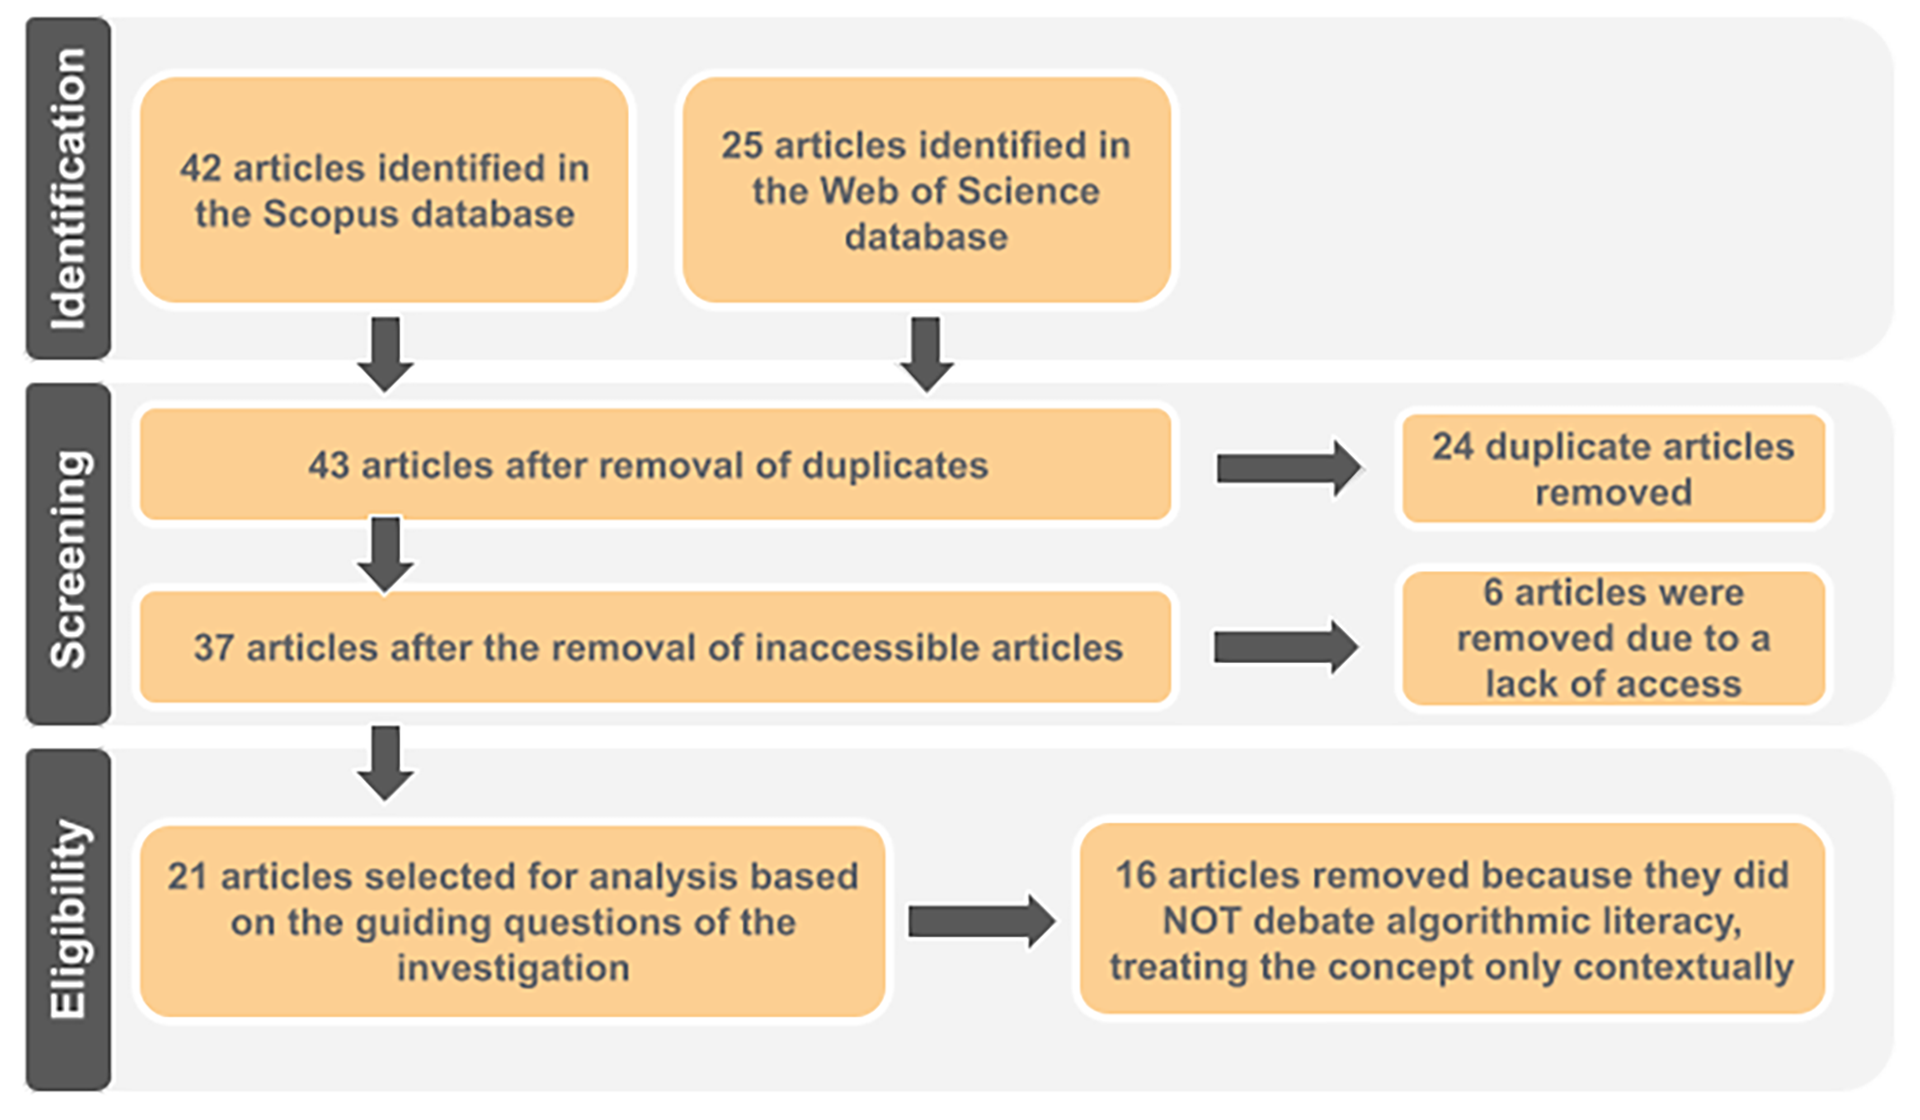
\includegraphics[width=\linewidth]{image1_en.png}
\source{Created by the authors.}
\end{minipage}
\end{figure}

In the screening phase, 24 duplicate publications were identified, that is, studies that appeared on both search platforms. Furthermore, during the screening, six publications were considered inaccessible by the researchers. These works could not be obtained for different reasons: subscription restrictions, payment on certain platforms, or unavailability of the full text by the authors or magazines. The decision to remove these inaccessible publications was made based on the need to ensure the reliability and completeness of the review, as the inability to access the full content could negatively affect the analysis and interpretation of results.

After identifying and removing duplications and inaccessible publications, 37 articles remained for the eligibility phase. At this stage, inclusion and exclusion criteria become essential. Such definitions are established to ensure that the analytical focus of the guiding questions is reflected in the selection of publications, providing greater clarity and efficiency to the analysis process. As shown in \cref{tab-02}, the inclusion criteria include studies that address the concept of AL, as well as present proposals and reflections on practices intended to generate AL, in addition to articles written in Portuguese, English, or Spanish published up to the cut-off date of this review (December 2022). The exclusion criteria seek to eliminate studies whose full text was unavailable at the time of data collection, works unrelated to AL, and studies in which AL is addressed only as a contextual element for the analysis of a more specific theme.

   
\begin{table}[!htpb]
\centering
\begin{threeparttable}
\caption{Critérios de seleção para fase de elegibilidade}
\label{tab-02}
\begin{tabular}{p{0.475\textwidth} p{0.475\textwidth}}
\toprule
Inclusion criteria & Exclusion criteria \\
\midrule
Studies that address the concept of AL. & Studies that did not have the full text available to researchers at the time of data capture. \\
Studies that present proposals and reflections on practices intended to generate AL. & Studies that are not related to AL. \\
Articles written in Portuguese, English, or Spanish. & Studies in which AL is used only as a contextual element to analyze a more specific theme. \\
Publications available until the cut-off date of this review (December 2022). &  \\
\bottomrule
\end{tabular}
\source{Created by the authors.}
\end{threeparttable}
\end{table}   


In the Eligibility stage, the analysis process consisted of a thorough reading of the texts of the publications, together with the production of summaries about each study and its main findings. From these summaries and the original texts, the eligibility analysis was conducted. The most preponderant exclusion criterion was the elimination of publications that do not deepen the discussion on the concept of algorithmic literacy or do not present training or pedagogical proposals related to the topic (in total, 16). In these publications, algorithmic literacy appears as a side discussion, generally acted as an imperative for contemporary education, without substantially exploring its meaning or possible applications. We can cite the article by \textcite[p. 759]{Cotter2020}, which analyzes how the socioeconomic context continues to shape the use of digital technologies and deepen disparities, which indicates that “greater algorithmic literacy can also imply familiarity with the functioning of algorithms, as well as the ability to evaluate their informative results”. Although they highlight the relevance of algorithmic literacy, there is no debate about what exactly comprises this concept. Similarly, \posscite{Kapsch2022} article, which explores how young adults make sense of and reflect on their agency as users in relation to algorithms, sees algorithmic literacy as a possible result of the study's methodological proposal, without actually outlining a systematic definition. Still in this group of works eliminated in the eligibility phase, there are a series of studies that place AL as a tool for learning mathematics and computing \cite{Astambayeva2021,How2022}, an approach that distances itself from the objectives and issues guiding our study.

\section{Analysis}\label{sec-análise}

In this section, we will analyze the 21 articles selected for the systematic literature review on the concept of AL. All of the analyzed articles are detailed in a table in Annex I, which includes the name of the authors, year of publication, title of the article, type, and place of publication. We will first present an analysis of the publications' metadata, including the year of publication, authors, journals, or events in which they were presented, along with other relevant details. Next, we will effectively analyze the corpus, considering the questions that drive our investigation.

\subsection{Initial perspectives from metadata}

When analyzing the list of publications, we observed that the data covers a period of four years, from 2019 to 2022 \Cref{image-02}. Notably, most publications are concentrated in the years 2021 and 2022, in which 6 and 10 publications, respectively, were found. This concentration of debate on the concept of AL over the past four years, as well as the upward trend in the number of publications on the topic, may indicate increased recognition of the importance of understanding algorithms and their roles in contemporary social life, as well as the advancement of discussions surrounding AL.

\begin{figure}[!h]
\centering
\begin{minipage}{0.85\linewidth}
\caption{Number of publications per year.}
\label{image-02}
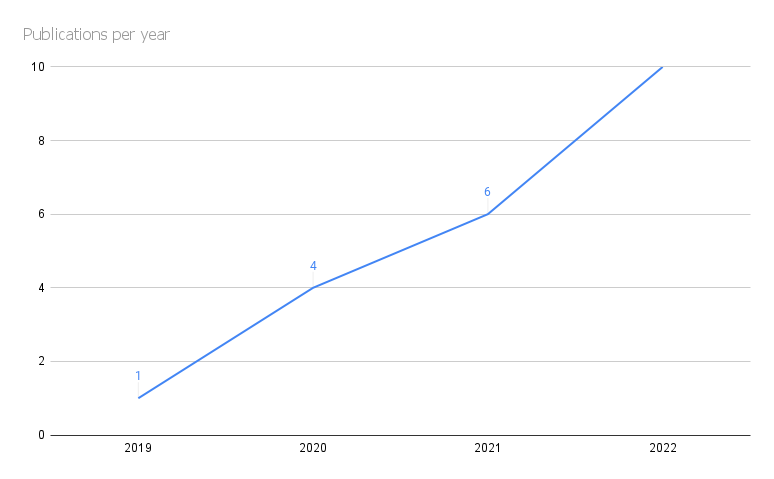
\includegraphics[width=\linewidth]{image2_en.png}
\source{Created by the authors.}
\end{minipage}
\end{figure}

Regarding the origin of the publications, it is possible to observe a diversity of formats, covering articles in periodicals (15), book chapters (2), and articles in the annals of academic events (4). As seen in the table in \Cref{anexo-1}, only two journals contain more than one article on the topic (AI and Society and Computers and Composition). It is noted that the studies found cover a wide range of areas: communication, computing, psychology, information science, education, in addition to other disciplines related to the debate on information and communication technologies (such as Human-Computer Interaction). This aspect may indicate the multidisciplinary interest in the topic and the relevance of the notion of AL in different academic contexts.

At this stage of the analysis, the absence of texts in Portuguese and the low number of publications in Spanish were also noticed among the 21 articles selected for the systematic review on AL. This observation may indicate a scenario of scarcity of investigations on the topic in the Latin and Ibero-American context.

With this information as a basis, the next stage of our analysis provides a more in-depth study of these publications, considering the guiding questions of the investigation on conceptual proposals, pedagogical techniques, practical applications, and difficulties related to AL.

\subsection{Exploring the foundations of Algorithmic Literacy (AL): conceptual models, distinctions, and multidisciplinary applications}

The analysis of articles that address AL reveals a diverse and complex scenario, in which no conceptual unity is observed. It was first noted that the debate surrounding AL has proposals that derive from pre-existing and more consolidated literacy approaches, such as information literacy, literacy for the digital environment, and data literacy \cite{Lloyd2019}. These approaches emphasize the process of creating individual awareness on how information is produced, classified, and distributed in different environments \cite{Bakke2020}. In these studies, AL emerges as a response to the effects of the introduction of algorithmic agency, a series of more specific skills in the scenario of a datafied life \cite{Kampa2021}. In this context, calls for literacies are often a response to new technologies that create new power structures \cite{Devito2021}.

For \textcite[p. 3]{Ridley2021}, AL is one of the offshoots of the varied literacies of the digitalized world: “Although each of them has its own domain and focus, they share common ideas and are generally symbiotic with each other”. Similarly, \textcite[p. 30]{Devito2021} argues that AL should not be observed in isolation, but rather as “a component of a broader platform literacy that encompasses all of the literacies mentioned previously”. For \textcite{Lloyd2019}, what differentiates AL from more general literacy proposals is that it requires an in-depth examination of the development culture of these systems, a movement that is in line with research proposals, such as that of \textcite{Seaver2017}. “According to this perspective, building an algorithm is a practice that is embedded within other practices and is influenced by specific views of the world” \cite[p. 1483]{Lloyd2019}.

In this context, the specificity of AL in relation to other digital pedagogical approaches lies in the need for a critical examination of characteristic properties of algorithmic agency, based on notions such as performativity, opacity, diversity, trust, bias, and social justice \cite{Lloyd2019}. In addition, \textcite{Devito2021} indicates that any AL proposal must deal with the unstable nature of algorithmic systems in constant transformation, incorporating this flexibility and ability to update into pedagogical constructions. For the author, this makes it essential to recognize that “subjects are already immersed in the environment in question, making AL an exercise mainly to formalize and correct the knowledge found in the world, rather than introducing purely new knowledge” \cite[p. 3-4]{Devito2021}.

In the analyzed studies, one of the main goals for AL is the development of awareness concerning the agency of algorithmic systems in different interactions with subjects \cite{Bakke2020}, whether in the search for information and content \cite{Kampa2021}, in interaction with automated interaction systems \cite{Shin2022} or in relation to algorithmic personalization \cite{Devito2021,Lv2022,Bell2023}. According to \textcite{Ridley2021}, this is a way of recognizing and raising awareness about the forms of power of this technological standard and, at the same time, emphasizing the empowerment possible for subjects in the face of these structures. In this approach, LA can be defined as the ability to be aware of both the presence and developments of algorithmically driven systems and, thus, crystallize this understanding into a strategic use of these systems so that the subjects participating in this process can achieve individual or collective objectives \cite{Devito2021}. Therefore, AL should be understood as more than instructions for a more efficient use of algorithmic systems. It is an ideological practice of producing meaning and subjectivizations that are dissonant with what the performativity of these systems allows \cite{Ridley2021}.

In the next segment of this analysis item, two constituent dimensions of the debates that emerge from the examined articles will be explored. First, the meaning of the notion of critical empowerment will be discussed. After, the spectrum of different levels of awareness of subjects in relation to algorithmic systems will be addressed. Both debates are key to the conceptual AL proposals analyzed in our study.

\subsection{Critical empowerment: paths of agency in the face of algorithmic systems}\label{sub-sec-empoderamentocritico}

Power and control are two core notions in the debate established by the critical literature on algorithms. \textcite{Magalhaes2018} maintains that part of the literature, which he calls the damage paradigm, considers the power of algorithms as both a result and a driver of an original disparity between subjects (who have their lives affected by the analysis of digital data without being aware of it), and platform operators (who deliberately and strategically control the collection and analysis of this data). As \textcite{Rieder2018} indicates, these approaches are often geared towards simply denouncing the political and social effects of algorithmic systems, neglecting the analysis of how these infrastructures are articulated materially and discursively to produce the effects of power.

In analyzing the articles in the sample, it seems clear to us that power and control are issues for which the investigations analyzed seek to offer some type of answer or critical approach. In them, LA tends to be positioned as pedagogical knowledge for the development of critical consciousness and, consequently, the expansion of the subjects' agency capacity. It is in this context that the notion of critical empowerment emerges as an expected result of AL. In the conceptual proposals analyzed, there is an emphasis on individual empowerment based on the ability to critically observe the ways in which these systems function \cite{Bakke2020,Konig2022}.

\textcite{Konig2022}, for example, maintains that AL can form subjects with a reflective stance in relation to algorithmic systems, allowing them to understand that, with each suggestion or result generated by these systems, there are tractions of objectives, interests and assumptions that are not necessarily clear. Similarly, \textcite[p. 1483]{Lloyd2019} understands that reflection processes are central to literacies; thus, they can collaborate to generate attention on how “algorithms are expressed and operationalized (through our actions and interactions with interfaces and programs), along with the conditions, assumptions, and biases that are inherent in their production and operationalization”. \textcite[p. 177]{Sued2022} indicates that critical awareness and knowledge developed from AL can guarantee subjects “greater agency and freedom of action”.

However, warns \textcite{Konig2022}, critical empowerment as a result of AL proves to be limited for two reasons. First, the effect of a critical understanding of algorithms is naturally restricted, as there is no guarantee that people will be able to incorporate this knowledge and attitudes to exercise control over the operations of an algorithmic system. The configurations, interfaces, and rules of these systems often act to limit the possibilities for individual choice. Even if it is possible to grant users more control through individual influence over the configuration and behavior of the system, a second obstacle remains: the production of a more active and engaged stance of these subjects in the process of defining their objectives, interests, and values within these systems.

Therefore, in the debate about AL, the ability to develop a critical awareness in relation to algorithmic systems is seen as a way to expand the subjects' agency, a critical response. In this sense, in accordance with \posscite{Siles2024} approach, we consider that the debate on AL is intertwined with the notion of agency. When looking at what people do with algorithms, \textcite{Siles2024} proposes a more fluid agency approach, which derives from the bricolage between discussions in Cultural Studies and Science and Technology Studies. In this proposal, the relationship with algorithms comes to be seen less as solid opposite poles or definitive states and more as relationships of convergence, instability, coexistence, friction, and change. Sometimes users follow the algorithms' suggestions, other times they resist them. Often, they have both positions in the same actions. It is now considered that agency is a relational process that takes place in the intermediate space of the relationship between subjects and algorithms \cite{Siles2024}.

In the next item, reflections on the different levels of awareness about the functioning of algorithmic systems are discussed, a prominent point in the literature on the topic.

\subsection{Levels of awareness and perception about algorithms}

Awareness about the existence and functioning of algorithms is a recurring theme in discussions about digital platforms. Initial research, carried out in the middle of the previous decade, indicated a low level of awareness about the existence and functioning of algorithms \cite{Eslami2015}. \textcite{Bucher2019}, for example, investigated the way people become aware of algorithmic agency, suggesting that the imagination about the functioning of these systems can condition the way these individuals develop their practices on a given platform.

In the debates observed in our study, the subjects' perception of algorithms is positioned as a central factor in AL, based on the premise that the ways of understanding these systems can significantly shape the subjects' practices and interactions with their digital environments. In the studies observed in the analyzed sample, different approaches can be noted that dialogue with this issue. \textcite{Bell2023} point out that awareness about the functioning of algorithmic systems can vary dramatically in a similar group. In the study, it is indicated that the perception about algorithmic systems can vary between platforms and is usually more verbalized when talking about services in which personalization systems are more prominent in use, such as TikTok \cite{Bell2023}. According to the authors, this perception may even depend on the way the topic is presented to the subjects (for example, based on the variation in terms chosen, such as algorithm or personalization). Findings from \textcite{Lv2022} correlate this awareness with teenagers' intention to resist algorithms on online platforms. For the authors, the different levels of awareness and knowledge about algorithms are related to the willingness of adolescents to search for ways to deal with or avoid these systems \cite{Lv2022}. The study by \textcite[p. 352]{Parnell2022}, which analyzes queries to online search engines, presents empirical findings that indicate that “greater algorithmic literacy has a positive effect on self-reported skills in using search systems and a more frequent use of the Internet”.

In these studies, it is possible to perceive an effort to create parameters that make it possible to measure degrees of awareness and knowledge about algorithmic systems. These would be degrees of AL that can be identified based on the subjects' practices. One of the proposals that most advances this purpose is that of \textcite{Devito2021}. The author seeks to establish categories to stratify these different levels of consciousness and knowledge, which she calls the Levels of Complexity of Individual Theorization. The degrees of understanding observed by the author are developed, mainly, from folk theories, or informal theorizations, as a result of the subjects’ experience in their relationships with algorithmic systems and, at the same time, from contact with other content that addresses the topic. Such content becomes incorporated into the ways in which these subjects organize their practices \cite{Devito2021}.

The stratification proposed by the author is divided into two levels that each have subdivisions: the first is Functional Theorists, which portrays subjects who have initial awareness and limited understanding of the functional aspects of algorithms. This category is divided into Basic Awareness (when the subject identifies that an algorithmic system is in operation on a platform, having some effect, but does not affirm or cannot reflect on what specific effect) and Causal Powers (when the subject indicates that an algorithmic system is the cause of a given result). The second level is that of Structural Theorists, which highlights subjects who make substantial adjustments to their tactics in order to deal directly with algorithmic issues, expanding their sources of information. This category is divided by \textcite{Devito2021} into Mechanistic Fragments (when the subject indicates that an algorithmic system plays specific roles on a platform and believes that it has identified multiple factors that are weighted by the system to make decisions) and Mechanistic Ordering (when the subject perceives that an algorithmic system plays specific roles on a platform and believes that it has identified not only multiple factors used to make decisions, but also the order in which these criteria are applied or the relative weight of each of them).

Therefore, subjects' perception and knowledge about algorithms emerge as crucial issues in the context of AL. The literature analyzed demonstrates that the understanding of these systems can vary significantly between the subjects and the platforms observed, a variation that can considerably influence their interactions and digital practices. Furthermore, empirical research suggests that higher levels of awareness about algorithms are related to a greater willingness to create more strategic ways of interacting with these systems. The categorization proposed by \textcite{Devito2021} to stratify different levels of awareness and knowledge about algorithms offers an interesting approach to evaluating and understanding these differences. However, it is necessary to highlight the contingent role that individual uses and practices can have in the context of the relationship with algorithms, as well as the aforementioned unstable nature of these systems. These factors make any generalizing proposal about levels of perception and knowledge limited.

\subsection{Pedagogical proposals in the context of algorithmic literacy}\label{sub-sec-aspropostaspedagogicas}

The analysis developed in our study made it possible to observe in the articles studied a set of pedagogical proposals developed with the aim of promoting knowledge and awareness about the performance of algorithmic systems. It is interesting to note that the proposals observed do not form a methodologically uniform set. There are different paths for the development of AL, which are presented below.

When trying to systematize the methodological paths of AL \textcite{Silva2022} indicate two possible paths. The first consists of building basic knowledge by exploring the objectives of the developers of these systems and the effects of these technologies on our societies. This approach, which we classify as content-based, is developed by offering solid information about the underlying purposes of algorithms and how they affect different dimensions of everyday life. The second path focuses on the production of experience through interaction with algorithmic systems. In this case, learners are encouraged to explore the functionalities of the algorithms, seeking to develop their schemes and knowledge to explain how they work and how their decisions are made.

Exploring the experiences developed by subjects in contact with algorithmic systems is also a central pedagogical proposal of \posscite{Devito2021} study. As already highlighted, the author focuses her discussion on folk theories to “explain the results, effects, or consequences of technological systems” \cite[p. 4]{Devito2021}. This proposal is premised on the notion that we already have, to a greater or lesser extent, some experience with these systems, therefore AL should be primarily the exercise of formalizing and correcting knowledge found in the world, rather than purely introducing new knowledge \cite{Devito2021}. The methodological purpose of AL defended by \textcite{Devito2021} is to develop learning modes that lead subjects to a structural understanding of these systems. This involves both understanding that algorithms have an effect on specific outcomes and identifying the various specific factors that are weighted by the algorithms and the order in which these criteria are applied.

\textcite{Ridley2021} rely on the literature concerning computational thinking to develop pedagogical proposals in the field of AL. For the authors, these two notions have an interesting correlation and, therefore, the extensive literature on computational thinking is considered by them as fruitful for AL \cite{Ridley2021}. The authors consider that such an approach can help develop an understanding of algorithms and their processes, interpret their uses in different systems, and create and apply algorithmic techniques and tools to solve problems in a variety of domains.

On the path of pedagogical development based on experiences, \textcite{Klumbbyte2020} discuss the promotion of AL through pedagogical approaches that use critical design for interaction with algorithms. The authors' proposal centers on the idea of developing the Social Privilege Estimator, a social scoring system based on facial recognition and classification, which was built as a critical design artifact to raise awareness about existing inequalities and the adverse effects of security systems of facial recognition. Moreover, in the field of design, \textcite{Cech2020} proposes a debate on co-design measures to support the development of AL and the understanding of algorithmic processes. Through participatory and user-centered design principles, the author suggests the collaborative design of material and procedural solutions to understand algorithmic and promotional processes in these systems.

Finally, we observed proposals that establish what we call narrative interaction as a method for developing AL: pedagogical methodologies that are based on the development of experiences based on narrative proposals, such as games and dynamics, in which subjects are invited to act and make decisions as if they were developers of these systems. \textcite[p. 199]{Aleman2021} present the proposal for a digital game in which subjects are placed in interaction with “an engaging narrative and a programming environment that demonstrate the limitations of predictive models”. The authors' proposal seeks to lead educators and students to examine the biases of algorithmic models, thus  encouraging reflection on the tensions with algorithmic systems in their lives.

In a similar way, \textcite{Jeong2022} propose the implementation of educational initiatives, focusing on the YouTube recommendation system based on a dynamic that seeks to place elementary school students in the shoes of the algorithm, as responsible for defining what is relevant on the platform. The authors' proposal is inspired by the methodology developed by \textcite{Grosman2022}, which consists of a dynamic that offers participants data and objectives for making musical suggestions on YouTube. According to \textcite{Jeong2022}, the proposal aims to encourage young people to understand how recommendation algorithms work and affect their interactions with YouTube.

Still in the context of the classroom, \textcite{Koenig2020} proposes textual production in diaries as a pedagogical methodology to encourage students' reflections on their interactions with platforms. The author's proposal basically consists of creating individual diaries to explore and reflect on their own interactions with algorithmic systems. It encourages reflection on students’ experiences with platforms based on textual production about experiences and habits. From the empirical experiment conducted, \textcite{Koenig2020} indicates that students have become more critical and aware of how platforms work.

The analysis of the pedagogical proposals indicates that there are different methodological paths that seek to promote knowledge and awareness about the performance of algorithmic systems. The proposals observed can range from more traditional, content-based approaches, in which the aim is to inform subjects about the action of algorithms, to more relational approaches, in which subjects are invited to experience new ways of interacting with these systems.

\section{Final considerations}\label{sec-consideraçõesfinais}

Our study aimed to map the field of research on AL in Portuguese, Spanish, and English. For this, four axes were used: the definition of conceptual proposals, the identification of emerging pedagogical techniques and strategies, the description of the functions and domains of these different forms of knowledge, and the reflection on the challenges and difficulties revealed in the literature.

Regarding conceptual proposals (Q1), we observed a diverse set of approaches, which, although they make references to pre-existing literacies, have specificities that differentiate them. In general, what differentiates AL from predecessor literacy proposals is the critical focus on the agency of algorithmic systems, considering their performative and changeable nature.

As for pedagogical approaches (Q2), despite the limited number of publications on the topic, a diversity of strategies around teaching and awareness about algorithms is perceived. Among these approaches, content methodologies stand out, which seek to inform subjects about the consequences of the relationship with algorithms, as well as experiential methodologies, which encourage the exploration of experiences and knowledge developed in interactions with algorithmic systems. Proposals for critical design, interaction in games, textual production, and narrative dynamics also emerge as methodologies that aim to involve subjects in the process of understanding and criticism.

Regarding the areas of knowledge in which the debates on AL are located (Q3), it is possible to affirm that it is an eminently transdisciplinary research object. In our study, we noticed a significant breadth of fields of knowledge in which the topic has been studied, such as communication, computing, education, psychology and information science. Regarding the difficulties perceived in the analyzed studies (Q4), we consider that the central challenge for the field of investigation is the lack of a clear and consistent definition of the concept, along with its proximity to other forms of literacy. Regarding the development of critical consciousness, the studies analyzed refer to difficulties related to the often opaque and complex nature of algorithmic systems, especially regarding understanding and agency over their functioning and developments. Difficulties are also referred to as inequalities in access to digital technologies.

In conclusion, AL is an emerging and transdisciplinary area that needs development, both conceptually, for greater clarity, and methodologically, with the development of proposals that can assist in the process of promoting awareness and critical thinking regarding the actions of algorithms. We can place it as a series of knowledge and dynamics that aim to produce awareness about the agency of algorithms in relationships and that are established in the environments of platforms. The different approaches to AL commonly provide ways in which subjects can strategically use these systems to achieve personal and collective goals. Unlike other forms of literacy, AL requires a critical examination of the development practices of algorithmic systems, addressing issues such as performativity, opacity, bias, and social justice.


\printbibliography\label{sec-bib}
%conceptualization,datacuration,formalanalysis,funding,investigation,methodology,projadm,resources,software,supervision,validation,visualization,writing,review
\begin{contributors}[sec-contributors]
\authorcontribution{Willian Fernandes Araujo}[conceptualization,methodology,writing,review]
\authorcontribution{Fernanda Pires de Sá}[methodology,writing]
\end{contributors}

\appendix
\section*{Anexo}\label{anexo-1}

\setlength\LTleft{-0.8in}
\setlength\LTright{-0.8in}
\begin{footnotesize}
\begin{longtable}{
    >{\raggedright\arraybackslash}p{0.2\textwidth}
    >{\raggedright\arraybackslash}p{0.075\textwidth}
    >{\raggedright\arraybackslash}p{0.4\textwidth}
    >{\raggedright\arraybackslash}p{0.125\textwidth}
    >{\raggedright\arraybackslash}p{0.2\textwidth}
    }
\caption{Local de publicação de acordo com área de concentração e natureza} \label{tab-anexo-1}\\
\\
\toprule
Autores(as) & Ano & Título do texto &Tipo &Fonte da publicação\\
\midrule
Lloyd, A. & 2019 & Chasing Frankenstein's monster: information literacy
in the black box society & Artigo em Periódico & Journal of
Documentation \\
Bakke, A. & 2020 & Everyday Googling: Results of an Observational Study
and Applications for Teaching Algorithmic Literacy & Artigo em Periódico
& Computers and Composition \\
Cech, F. & 2020 & Beyond transparency: Exploring algorithmic
accountability & Texto publicado em anais de eventos & Proceedings of
the International ACM SIGGROUP Conference on Supporting Group Work \\
Klumbyte, G.; Lücking, P.; Draude, C. & 2020 & Reframing AX with
Critical Design: The Potentials and Limits of Algorithmic Experience as
a Critical Design Concept & Texto publicado em anais de eventos & 11th
Nordic Conference on Human-Computer Interaction: Shaping Experiences,
Shaping Society (NordiCHI '20), \\
Koenig, A. & 2020 & The Algorithms Know Me and I Know Them: Using
Student Journals to Uncover Algorithmic Literacy Awareness & Artigo em
Periódico & Computers and Composition \\
Aleman, E.; Nadolny, L.; Ferreira, A.; Gabetti, B.; Ortíz, G.;
Zanoniani, M. & 2021 & Screening bot: A playground for critical
algorithmic literacy engagement with youth & Texto publicado em anais de
eventos & CHI PLAY 2021 - Extended Abstracts of the 2021 Annual
Symposium on Computer-Human Interaction in Play \\
DeVito, M.A. & 2021 & Adaptive Folk Theorization as a Path to
Algorithmic Literacy on Changing Platforms & Artigo em Periódico &
Proceedings of the ACM on Human-Computer Interaction \\
Kampa, P.; Balzer, F. & 2021 & Algorithmic literacy in medical students
-- results of a knowledge test conducted in Germany & Artigo em
Periódico & Health Information and Libraries Journal \\
Reisdorf, B.C.; Blank, G. & 2021 & Algorithmic literacy and platform
trust & Capítulo de livro & Handbook of Digital Inequality \\
Ridley, M.; Pawlick-Potts, D. & 2021 & Algorithmic literacy and the role
for libraries & Artigo em Periódico & Information Technology and
Libraries \\
Swart, J. & 2021 & Experiencing Algorithms: How Young People Understand,
Feel About, and Engage With Algorithmic News Selection on Social Media &
Artigo em Periódico & Social Media and Society \\
Bell, A.R., Tennfjord, M.K., Tokovska, M., Eg, R. & 2022 & Exploring the
role of social media literacy in adolescents\textquotesingle{}
experiences with personalization: A Norwegian qualitative study & Artigo
em Periódico & Journal of Adolescent and Adult Literacy \\
Dogruel, L., Masur, P., Joeckel, S. & 2022 & Development and Validation
of an Algorithm Literacy Scale for Internet Users & Artigo em Periódico
& Communication Methods and Measures \\
Jeong, H.-S., Oh, Y.J., Kim, A. & 2022 & CRITICAL ALGORITHM LITERACY
EDUCATION IN THE AGE OF DIGITAL PLATFORMS: Teaching children to
understand YouTube recommendation algorithms & Capítulo de livro &
Learning to Live with Datafication: Educational Case Studies and
Initiatives from Across the World \\
König, P.D. & 2022 & Challenges in enabling user control over
algorithm-based services & Artigo em Periódico & AI and Society \\
Lv, X., Chen, Y., Guo, W. & 2022 & Adolescents' Algorithmic Resistance
to Short Video APP's Recommendation: The Dual Mediating Role of
Resistance Willingness and Resistance Intention & Artigo em Periódico &
Frontiers in Psychology \\
Parnell, S.I., Klein, S.H., Gaiser, F. & 2022 & Do we know and do we
care\textquotesingle{} Algorithms and Attitude towards Conversational
User Interfaces: Comparing Chatbots and Voice Assistants & Texto
publicado em anais de eventos & 4th Conference on Conversational User
Interfaces (CUI 2022) \\
Shin, D. & 2022 & How do people judge the credibility of algorithmic
sources? & Artigo em Periódico & AI and Society \\
Shin, D., Rasul, A., Fotiadis, A. & 2022 & Why am I seeing this?
Deconstructing algorithm literacy through the lens of users & Artigo em
Periódico & Internet Research \\
Silva, D.E., Chen, C., Zhu, Y. & 2022 & Facets of algorithmic literacy:
Information, experience, and individual factors predict attitudes toward
algorithmic systems & Artigo em Periódico & New Media and Society \\
Sued, G.E. & 2022 & TRAINING THE ALGORITHM: GOVERNANCE, AGENCY, AND
LITERACY IN THE USE OF YOUTUBE {[}Entrenar al algoritmo: gobernanza,
agencia y literacidad en el uso de YouTube{]} & Artigo em Periódico &
Contratexto \\
\bottomrule
\source{Elaboração própria.}
\end{longtable}
\end{footnotesize}


\end{document}
